\section{Experiments}\label{sec:experiments}

We first check each mechanism in isolation, then measure the contribution of every layer on a randomized paired benchmark (\cref{sec:results}), isolate the gap search, the coordination and the CBF by ablation (\cref{sec:ablation}), and finally report what a live Nav2 deployment confirms and exposes (\cref{sec:live}).

\subsection{Experimental Setup}\label{sec:setup}

\noindent\textbf{Evaluation Surface.} The controlled quantitative comparison is a randomized 2D benchmark that reuses the controller's primitives in NumPy and OSQP: the MPPI sampler, the APF repulsion, the gap raycast, the look-ahead-point CBF-QP, the $\alpha$ coordination with TTC override, and the monotone-progress entrapment detector. As in the released controller and the deployment lesson of \cref{sec:live}, the CBF and the TTC see only the dynamic obstacles, never static walls. The 2D mirror is not the live Nav2 controller: it drives a 2D unicycle, uses distance-to-goal progress and a free-space gap subgoal in place of a global path, and certifies the look-ahead point rather than the full body; \cref{app:mirror} lists every difference. We use this surface instead of a live Gazebo matrix because on the only host available to us (a WSL2 workstation running at a real-time factor of about $0.3$--$0.6$ under CPU contention, with transform smear adding phantom cells to the costmap) a live comparison measures the host rather than the algorithm.

\noindent\textbf{Scenario Families.} Four seed-deterministic families exercise the two weaknesses and their conjunction. \emph{U-trap}: a finite U- or C-shaped pocket with the goal behind its back wall, a static local minimum. \emph{Clutter}: a random field of 5--9 circular obstacles with a guaranteed footprint-clear path. \emph{Dynamic}: one or two pedestrian-like movers timed to cross the robot's path. \emph{Narrow-dynamic}: the U-trap pocket plus movers sweeping its mouth during the escape window, the narrow-and-dynamic coincidence the coordination targets.

\noindent\textbf{Configurations.} Six ablation configurations toggle the mechanisms: \textbf{A}~stock MPPI (no escape, no CBF); \textbf{C}~escape only; \textbf{D}~CBF only; \textbf{E}~escape+CBF with $\alpha_{\mathrm{escape}}=\alpha_{\mathrm{base}}$, i.e.\ independent layers; \textbf{F}~full \sname{} with $\alpha:2\to6$ and TTC override, i.e.\ coordinated; and \textbf{F$^{-}$}~F with the gap search disabled. The deployable baselines of the specified full-scale protocol (DWB, RPP, TEB, a DRPA-style always-on escape and a Shield-style CBF-only controller) have not been run; we make no comparison to them.

\noindent\textbf{Protocol and Metrics.} Every scenario is a pure function of an integer seed, and the MPPI noise stream uses the same seed, so all configurations face byte-identical worlds and rollout noise, as the paired design requires. We run $4$ families $\times$ $50$ seeds $\times$ $6$ configurations $=1{,}200$ trials with a budget of $400$ steps of $0.1$\,s. A trial is a success if it reaches the goal without a footprint collision, a collision if the footprint overlaps an obstacle, and a timeout otherwise. Success carries a Wilson 95\% interval; the primary test is McNemar on paired outcomes; continuous metrics (time-to-goal, path length, clearance) use Mann--Whitney $U$ with Cliff's $\delta$; all $p$-values are Holm-corrected within each family (16 tests per family). The benchmark runs on CPU in Python; we report no per-cycle compute figures (\cref{sec:discussion}). Parameters are in \cref{tab:params}, and commands in \cref{app:repro}.

\subsection{Main Results}\label{sec:results}

\begin{figure}[t]
\centering
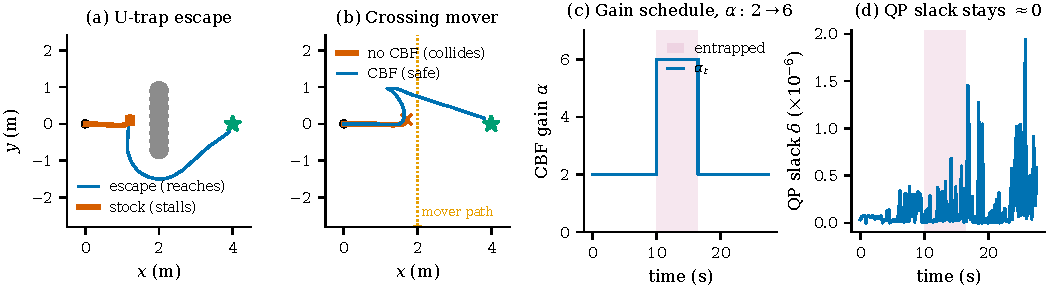
\includegraphics[width=\linewidth]{figures/mechanism.pdf}
\caption{\textbf{Mechanism validation in the 2D mirror} (seed-fixed single runs; \cref{tab:mechanism}). \textbf{(a)}~Stock MPPI stalls at the mouth of a finite wall ($x\approx1.2$\,m) while the detection-and-escape layer rounds it to the goal. \textbf{(b)}~Against a mover crossing the path, the no-CBF controller collides ($\times$) while the look-ahead-point CBF filter keeps the robot clear. \textbf{(c,\,d)}~On the U-trap, the coordinated gain rises from $\alpha_{\mathrm{base}}{=}2$ to $\alpha_{\mathrm{escape}}{=}6$ while entrapped (shaded) and the QP slack stays below $2\times10^{-6}$ throughout: the escape is admitted without relaxing the barrier, close to the slack-free setting that \cref{prop:invariance} assumes. Regenerated as vector graphics by \texttt{scripts/make\_figures.py}.}
\label{fig:mechanism}
\end{figure}

\begin{table}[t]
\centering
\caption{\textbf{Mechanism validation} (single seed-fixed runs of the 2D mirror; 40\,s budget). ``Stalled'' = budget exhausted without progress. Source: \texttt{data/mechanism\_validation.json}, regenerated from \texttt{experiments/prototype/run\_validation.py}.}
\label{tab:mechanism}
\small
\begin{tabular}{llccccc}
\toprule
Scenario & Configuration & Reached & Collided & Time (s) & Min.\ clear.\ (m) & $\max_t\alpha_t$ \\
\midrule
U-trap & stock MPPI (A) & no (stalled) & no & -- & 0.33 & 2 \\
U-trap & escape (C) & yes & no & 27.7 & 0.32 & 2 \\
Crossing mover & escape, no CBF (C) & no & yes & -- & $-$0.00 & 2 \\
Crossing mover & \sname{} (F) & yes & no & 18.6 & 0.01 & 6 \\
U-trap & \sname{} (F) & yes & no & 27.7 & 0.32 & 6 \\
U-trap + mover & independent (E) & yes & no & 27.7 & 0.32 & 2 \\
\bottomrule
\end{tabular}
\end{table}


\noindent\textbf{Mechanism Check.} Before measuring rates, we verify that each mechanism does what it is designed to do on three hand-built scenes (\cref{fig:mechanism}, \cref{tab:mechanism}). Stock MPPI stalls in front of a finite wall for the full $40$\,s budget, while the escape layer reaches the goal in $27.7$\,s; against a crossing mover the no-CBF controller collides after $4.7$\,s, while the CBF filter reaches the goal in $18.6$\,s with the minimum clearance never negative; and on the U-trap the coordinated gain rises from $2$ to $6$ while entrapped, with QP slack below $2\times10^{-6}$ throughout, so the escape is admitted without relaxing the barrier (\cref{prop:invariance}). In these benign scenes the coordinated and independent variants are both safe and equally fast ($27.7$\,s, $0.32$\,m clearance), so they cannot separate the two; the randomized benchmark below is the quantitative test.

\begin{table}[t]
\centering
\caption{\textbf{Main result: success rate} in \% with Wilson 95\% confidence interval, $N=50$ paired scenarios per cell ($1{,}200$ trials of the Python 2D mirror, not the Nav2 controller). Best per family in bold. On the two trap families the escape configurations (C, E, F) separate from stock (A), CBF only (D) and the no-gap ablation (F$^{-}$), which all stay at $0\%$. Source: \texttt{experiments/results\_2d/summary.csv}.}
\label{tab:main}
\small
\begin{tabular}{lcccc}
\toprule
Configuration & U-trap & Clutter & Dynamic & Narrow-dyn. \\
\midrule
A\,stock MPPI & 0\,{\scriptsize[0,7]} & 52\,{\scriptsize[39,65]} & 80\,{\scriptsize[67,89]} & 0\,{\scriptsize[0,7]} \\
C\,escape only & \textbf{90}\,{\scriptsize[79,96]} & \textbf{62}\,{\scriptsize[48,74]} & 76\,{\scriptsize[63,86]} & \textbf{78}\,{\scriptsize[65,87]} \\
D\,CBF only & 0\,{\scriptsize[0,7]} & 52\,{\scriptsize[39,65]} & 82\,{\scriptsize[69,90]} & 0\,{\scriptsize[0,7]} \\
E\,escape+CBF (indep.) & 88\,{\scriptsize[76,94]} & \textbf{62}\,{\scriptsize[48,74]} & 78\,{\scriptsize[65,87]} & 64\,{\scriptsize[50,76]} \\
\textbf{F\,\sname{} (coord.)} & 88\,{\scriptsize[76,94]} & \textbf{62}\,{\scriptsize[48,74]} & 78\,{\scriptsize[65,87]} & 62\,{\scriptsize[48,74]} \\
F$^{-}$\,F without gap search & 0\,{\scriptsize[0,7]} & 52\,{\scriptsize[39,65]} & \textbf{84}\,{\scriptsize[71,92]} & 0\,{\scriptsize[0,7]} \\
\bottomrule
\end{tabular}
\end{table}

\begin{table}[t]
\centering
\caption{\textbf{Paired contrasts against F} (McNemar on success, Holm-adjusted within each family of 16 tests). $b$ = trials the baseline solves and F does not; $c$ = the reverse. $^{*}$ marks $p_{\mathrm{adj}}<0.05$. The escape contrast (A$\to$F) is decisive on both trap families; the coordination contrast (E$\to$F) is null everywhere. Source: \texttt{experiments/results\_2d/stats.json}.}
\label{tab:contrasts}
\small
\begin{tabular}{lcccccc}
\toprule
 & \multicolumn{2}{c}{Escape (A$\to$F)} & \multicolumn{2}{c}{CBF cost (C$\to$F)} & \multicolumn{2}{c}{Coordination (E$\to$F)} \\
\cmidrule(lr){2-3}\cmidrule(lr){4-5}\cmidrule(lr){6-7}
Family & $b/c$ & $p_{\mathrm{adj}}$ & $b/c$ & $p_{\mathrm{adj}}$ & $b/c$ & $p_{\mathrm{adj}}$ \\
\midrule
U-trap & 0/44 & $1.4\!\times\!10^{-9}$$^{*}$ & 1/0 & 1 & 0/0 & 1 \\
Clutter & 0/5 & 1 & 0/0 & 1 & 0/0 & 1 \\
Dynamic & 3/2 & 1 & 1/2 & 1 & 0/0 & 1 \\
Narrow-dyn. & 0/31 & $1.1\!\times\!10^{-6}$$^{*}$ & 8/0 & 0.109 & 1/0 & 1 \\
\bottomrule
\end{tabular}
\end{table}


\noindent\textbf{The Escape Layer Is the Measured Contribution.} On both trap families the effect is decisive and survives Holm correction (\cref{tab:main,tab:contrasts}). Success rises from $0\%$, where stock A, CBF-only D and no-gap F$^{-}$ all time out in the pocket, to $88$--$90\%$ on U-trap (44 of 50 discordant pairs in F's favour, $p_{\mathrm{adj}}=1.4\times10^{-9}$) and to $62$--$78\%$ on narrow-dynamic (31 of 50, $p_{\mathrm{adj}}=1.1\times10^{-6}$). On clutter the escape adds $10$ percentage points ($52\%\to62\%$, not significant after correction) at the cost of about $2.4$\,s longer mean time-to-goal over successful trials ($15.2$\,s $\to$ $17.7$\,s; \cref{tab:full}). On the pure dynamic family, which contains no trap, it is appropriately neutral (A$\to$F: $b/c=3/2$, $p_{\mathrm{adj}}=1$). \Cref{fig:success} shows the full per-family picture, including collision and timeout rates.

\begin{figure}[t]
\centering
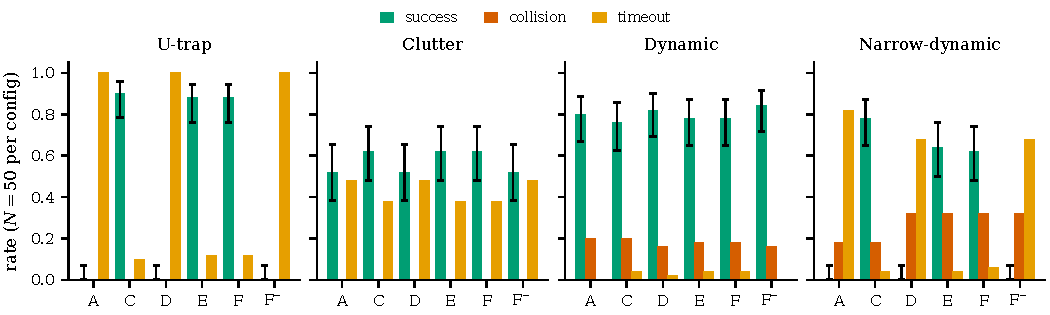
\includegraphics[width=\linewidth]{figures/success_bars.pdf}
\caption{\textbf{Outcome rates per family} across configurations A--F$^{-}$ ($N=50$ each; Wilson 95\% intervals on success). On the trap families (U-trap, narrow-dynamic) the escape configurations C, E and F separate from A, D and F$^{-}$, which time out at $0\%$ success. Plotted directly from \texttt{experiments/results\_2d/summary.csv}.}
\label{fig:success}
\end{figure}


\subsection{Ablation Studies}\label{sec:ablation}

\noindent\textbf{The Gap Search Is Load-Bearing.} F$^{-}$, which keeps the entrapment detector, the APF repulsion and the gain modulation but drops the gap search, scores $0\%$ on both trap families (\cref{tab:main}), identical to stock MPPI. Detection-and-switch escapes only \emph{with} the free-space gap subgoal: repulsion and gain modulation without a routed opening do not escape.

\noindent\textbf{Escape--Safety Coordination Is Null in This Regime.} The contrast that bears on the coordination contribution is E (independent) versus F (coordinated): identical mechanisms that differ only in whether the CBF gain follows the escape phase. Across all $200$ paired scenarios this contrast is null (\cref{tab:contrasts}, \cref{fig:evsf}): the discordant counts are $0/0$, $0/0$, $0/0$ and $1/0$, McNemar $p=1$ in every family, and every continuous effect size (Cliff's $\delta$) satisfies $|\delta|\le0.032$. The gain does engage as designed ($\max_t\alpha_t=6$ during escape, TTC override active). The per-trial slack telemetry (\cref{tab:slack}) locates where the barrier actually works. On the mover-free families the dynamic-obstacle CBF sees no obstacle at all: slack is zero in every trial, E and F issue identical commands, and the null there is structural. On narrow-dynamic the barrier \emph{does} engage and even relaxes, with nonzero slack in $34$ of $50$ trials for E and F ($26$ for D and F$^{-}$, maximum $0.47$), and on dynamic in $47$--$48$ of $50$ (maximum $0.015$); yet E and F still do not differ. The correct reading is therefore not that the barrier never binds, but that the \emph{outcomes are insensitive to the $\alpha$ schedule}: where the barrier is quiescent the two configurations coincide exactly, and where it is active both gains admit escapes whose outcomes are indistinguishable at $N=50$. In this benchmark the coordination produces no measurable outcome difference over independent escape+CBF. This is consistent with, and delimits, \cref{prop:invariance}: coordination is a certified-safe mechanism, not, in these scenarios, an outcome improvement.

\begin{figure}[t]
\centering
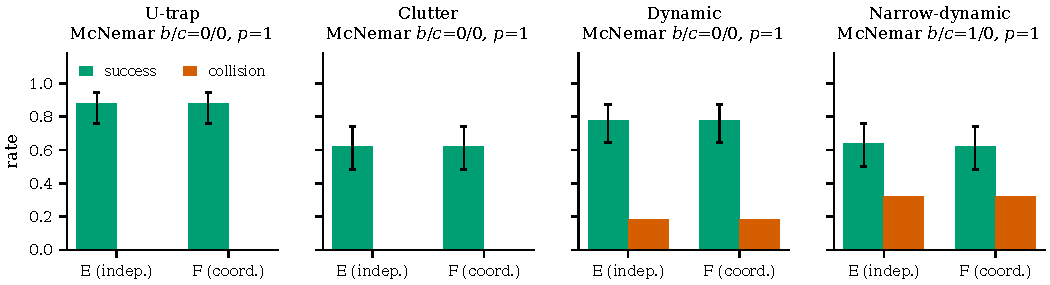
\includegraphics[width=\linewidth]{figures/e_vs_f.pdf}
\caption{\textbf{The coordination contrast is null.} Independent escape+CBF (E) versus coordinated \sname{} (F) per family, with the paired McNemar discordant counts and raw $p$-values from \texttt{experiments/results\_2d/stats.json}. The two are indistinguishable in every family.}
\label{fig:evsf}
\end{figure}


\noindent\textbf{What the CBF Changes.} Against body-grazing crossers (dynamic) the look-ahead-point filter leaves the collision rate essentially unchanged ($20\%$ for A versus $16$--$18\%$ with a CBF; descriptive, since the committed analysis carries no paired collision test). In the cramped narrow-dynamic pocket, the CBF configurations show a \emph{higher} collision rate than their no-CBF counterparts ($18\%\to32\%$, descriptive) and lose about $16$ points of success (C $78\%$ versus F $62\%$; McNemar $b/c=8/0$, raw $p=0.008$, $p_{\mathrm{adj}}=0.109$), which is directionally consistent though not significant after correction at $N=50$. We attribute both to the braking fallback and the point certificate and discuss them as limitations in \cref{sec:discussion}.

\subsection{Live Nav2 and Gazebo Integration}\label{sec:live}

We deployed \sname{} in a complete live stack: ROS~2 Jazzy, Nav2 (AMCL, costmaps, NavFn, behaviour-tree navigator, recovery, collision monitor) and the Gazebo \code{tb3_sandbox} world. The committed launch logs and trial telemetry confirm that the controller and the \code{EscapeCritic} load and activate from the critics list, that the controller produces velocity commands of the same form as stock MPPI, and that the lifecycle reaches the active state and sustains multi-minute drives on a U-trap testbed without a crash or collision after the fix below. The goal was not reached: the committed telemetry records STUCK at $254.5$\,s and TIMEOUT at $299.8$\,s, both collision-free, under the host constraints of \cref{sec:setup}. The escape-injection path has also run live: its first live activation exposed the ABI fault below, and the tensor shapes captured from that event are committed as a regression test, while the controller and critic now log every detection and injection transition for auditability. A sustained live entrapment-and-escape demonstration remains confounded by the host artefacts and is deferred to a GPU workstation. Three faults surfaced that only a live stack reveals:
\begin{itemize}
    \item \emph{Static walls in the CBF.} Feeding every lethal cluster, walls included, into the CBF makes the barrier infeasible everywhere and freezes the robot; scoping the CBF to moving, body-sized obstacles \eqref{eq:track} fixes it.
    \item \emph{Compute budget.} The per-cycle budget must match the host (horizon preserved, rate and batch reduced), or the loop misses its rate and the optimizer diverges.
    \item \emph{xtensor ABI mismatch.} The installed \code{libmppi_controller.so} is compiled with \code{XTENSOR_USE_XSIMD} and AVX2 (an aligned-allocator element type), whereas our plugin used the default allocator. Because the critic tensors cross the pluginlib boundary by reference, the first \code{EscapeCritic} write to \code{data.costs} violated the one-definition rule and crashed the whole Nav2 process on the first live escape injection. Unit tests could not catch it, since they compile every translation unit with one flag set, and earlier live runs had never triggered entrapment. Compiling the critic with the installed headers' flags, per target because a global AVX2 switch breaks the separately built OSQP--Eigen boundary, fixes it, and a regression test replays the injection with the live tensor shapes.
\end{itemize}
This is the class of fault a Nav2-native deployment exposes and that a standalone node or a pure 2D study cannot.
